\documentclass[12pt, french]{article}
\usepackage[french]{babel}
\selectlanguage{french}
\usepackage[T1]{fontenc}
\usepackage[utf8]{inputenc}
\usepackage{graphicx}
\usepackage{float}

% This is the preamble, load any packages you're going to use here
\usepackage{physics} % provides lots of nice features and commands often used in physics, it also loads some other packages (like AMSmath)
\usepackage{siunitx} % typesets numbers with units very nicely
\usepackage{enumerate} % allows us to customize our lists
\usepackage{array}


\begin{document}

\title{MI12 Projet : Analyse de mouvement Kinect/Smartphone}
\author{Matthieu Zins, Alexis Schad, Geoffrey Guyot}
\date{05/06/2016}


\maketitle

\section{Résumé}

L'objectif de ce projet est d'analyser un mouvement à partir de deux types de capteurs différents. Le premier est la Kinect qui permet de suivre le mouvement des mains de l'utilisateur. Le second est le capteur d'accélération intégré dans un téléphone. Par la suite, la mise en correspondance des données mesurées doit permettre de déterminer la main dans laquelle l'utilisateur tenait le téléphone.

\section{Exigences}

kinect 



\section{Principe}
L'utilisateur tient le smarphone dans une main et fait face à la Kinect. Une application Android lui permet de démarrer un enregistrement des accélérations du téléphone pendant une certaine période de temps. Du côté de l'ordinateur, un programme gère la Kinect et permet de suivre le squelette de l'utilisateur. Un troisième programme, également sur le PC, permet de contrôler les deux autres et de faire la mise en correspondance des mesures.

\begin{figure}[H]
\centering
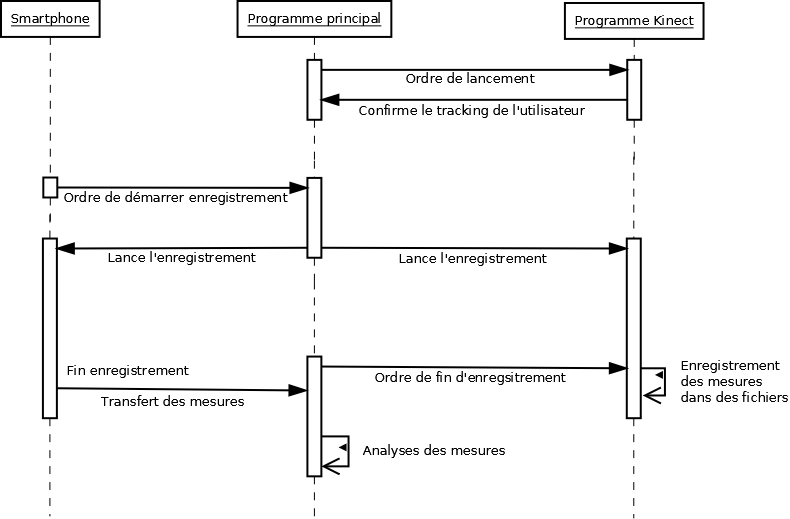
\includegraphics[scale=0.35]{diagramme_com.png}
\caption{Principe de fonctionnement}
\label{fig0}
\end{figure}

\section{Développement réalisé}

\subsection{Programme principal}
Ce programme permet de démarrer celui qui s'occupe de tracker l'utilisateur avec la Kinect et permet également de de démarrer un enregistrement.
Pour communiquer avec le PC, nous avons choisi d'utiliser le Bluetooth car il permet d'envoyer facilement des données vers le PC mais aussi au pc d'envoyer des ordres au téléphone.

Initialement, nous pensions réaliser ce programme en C++ avec la bibliothèque Qt, qui dispose d'une API Bluetooth. Une première version permettant de communiquer avec le téléphone a même été réalisée sur Linux. Cependant, nous nous sommes rendus compte que cette API Bluetooth n'est pas encore supportée sur Windows. Comme le programme gérant la Kinect tourne uniquement sur Windows, nous avons abandonné l'idée de réaliser le programme principal en C++. Nous avons donc choisi de le faire en python en utilisant la bibliothèque TKinter pour l'interface graphique et PyBluez pour la communication par Bluetooth.



\subsection{Application Android}
L'application développée permet de rechercher un appareil bluetooth à proximité et de s'y connecter. Une fois connectée, l'application permet à l'utilisateur de démarrer un enregistrement. Cela se traduit par une demande de démarrage envoyée au programme principal. Celui-ci vérifie que la Kinect "track" bien les deux mains de l'utilisateur puis envoie  l'ordre de démarrer l'enregistrement au téléphone et au programme gérant la Kinect.

L'enregistrement des données des capteurs se fait à une certaine fréquence. Android permet de régler la période d'échantillonnage. Cependant, comme indiqué dans la documentation Android, cette période n'est qu'une indication et n'est pas forcément respectée. Par exemple, voici les périodes d'échantillonnages lorsqu'on règle la période d'échantillonnage à 30 ms.

\begin{figure}[H]
\centering
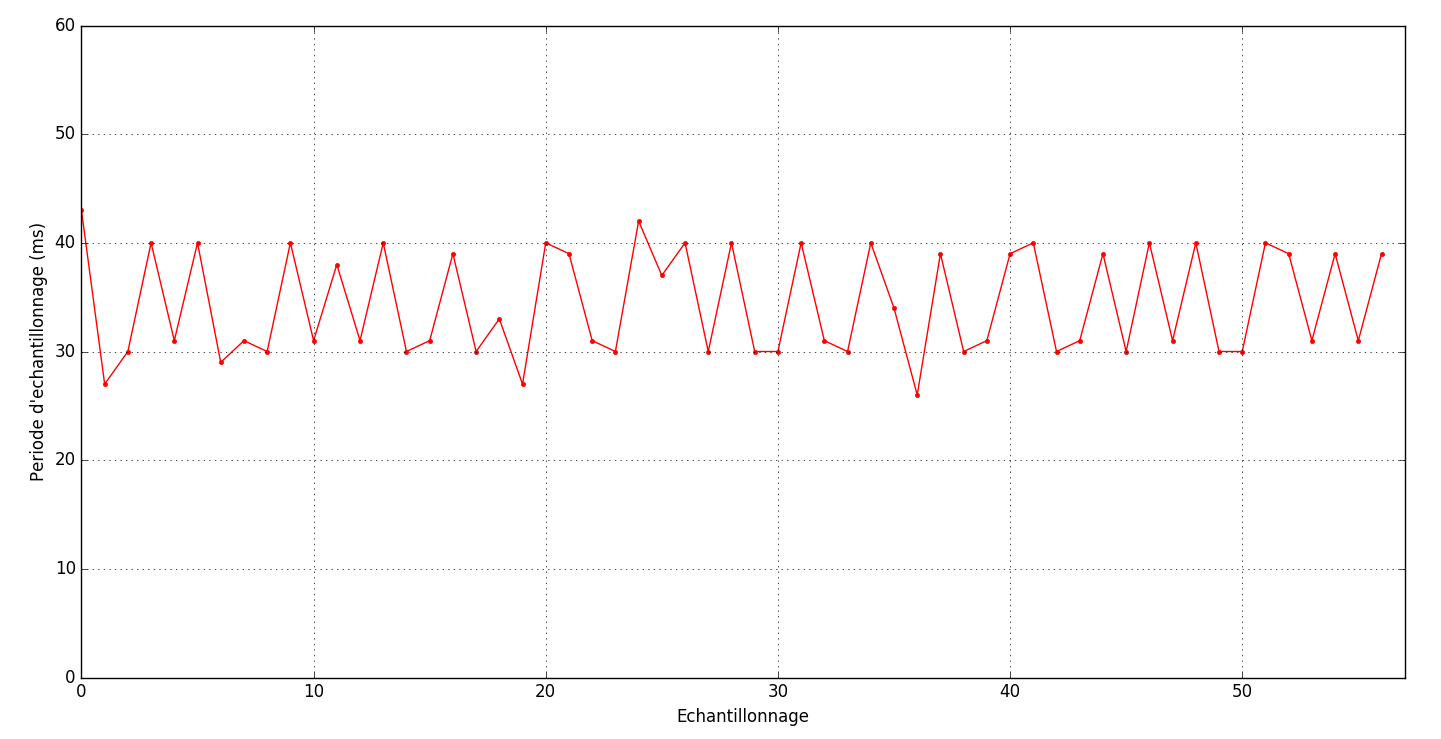
\includegraphics[scale=0.35]{sm_periode.png}
\caption{Période d'échantillonnage du téléphone}
\label{fig1}
\end{figure}


Android nous permet donc de récupérer les valeurs des accélérations subies par le téléphone suivant ses troix axes. Nous avons récupéré l'accélération linéaire qui est simplement l'accélération réelle à laquelle Android retire la gravité. Cependant cette accélération linéaire n'est pas pratique lorsqu'on fait un mouvement. En effet, pour obtenir les accélérations verticales et horizontales, il faudrait garder la même orientation du téléphone pendant tout le mouvement. Si le téléphone change d'orientation, l'accélération en z, par exemple, ne correspondra plus à l'accéleration verticale. Pour éviter cela, nous avons également récupéré, pour chaque mesure, une matrice de rotation définissant l'orientation du téléphone. Cette matrice permet de projeter les mesures d'accélérations du téléphone dans le repère "monde". Celui-ci est défini par :
\begin{itemize}
\item X qui est l'axe tangent au sol dirigé vers l'Est.
\item Y qui est l'axe tangent au sol dirigé vers le Nord.
\item Z  qui  est l'axe perpendiculaire au sol dirigé vers le ciel
\end{itemize}

\begin{figure}[H]
\centering
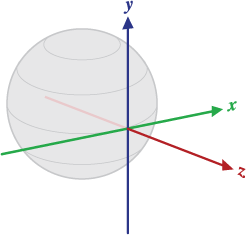
\includegraphics[scale=0.6]{axis_globe.png}
\caption{Repère "monde"}
\label{fig2}
\end{figure}

Lors de la phase de traitement des mesures, nous avons donc pu modifier le repère des accélérations. Cela se fait simplement en multipliant les mesures par la matrice de rotation en utilisant les coordonnées homogènes. 
\begin{figure}[H]
\[\left( 
\begin{array}{c}
Acc_x  \\
Acc_y  \\
Acc_z  \\
1 \end{array} 
\right)_{monde}=\qquad
\left( 
\begin{array}{cc}
Rot_{3x3} & 0  \\
0 & 1  \end{array} 
\right)*\left( 
\begin{array}{c}
Acc_x  \\
Acc_y  \\
Acc_z  \\
1\end{array} 
\right)_{tel}\]
\caption{Passage du repère "téléphone" au repère "monde"}
\end{figure}

Lors de l'enregistrement du mouvement, il faudra donc que l'utilisateur soit orienté face au Nord pour bien distinguer X et Y.




\subsection{Programme Kinect}
Ce programme permet de suivre les mouvements de l'utilisateur, notamment ses mains. Il a été développé en C++ avec les bibliothèques fournies par Microsoft permettant de récupérer les flux de la Kinect.
Pour communiquer avec le programme principal (en python), nous avons choisi d'utiliser un fichier mappé en mémoire. Ce type de mémoire partagée est accessible aux deux programmes et leur permet d'écrire ou de lire des octets de maniére presque instantanée. Le programme permet de "tracker" le squelette de l'utilisateur et peut enregistrer les positions successives de ses mains. Cependant, nous n'avons pas de réel de contrôle sur la fréquence des mesures. Sur la figure suivante, on peut voir que la période entre deux mesures varie entre 20 et 80 ms.

\begin{figure}[H]
\centering
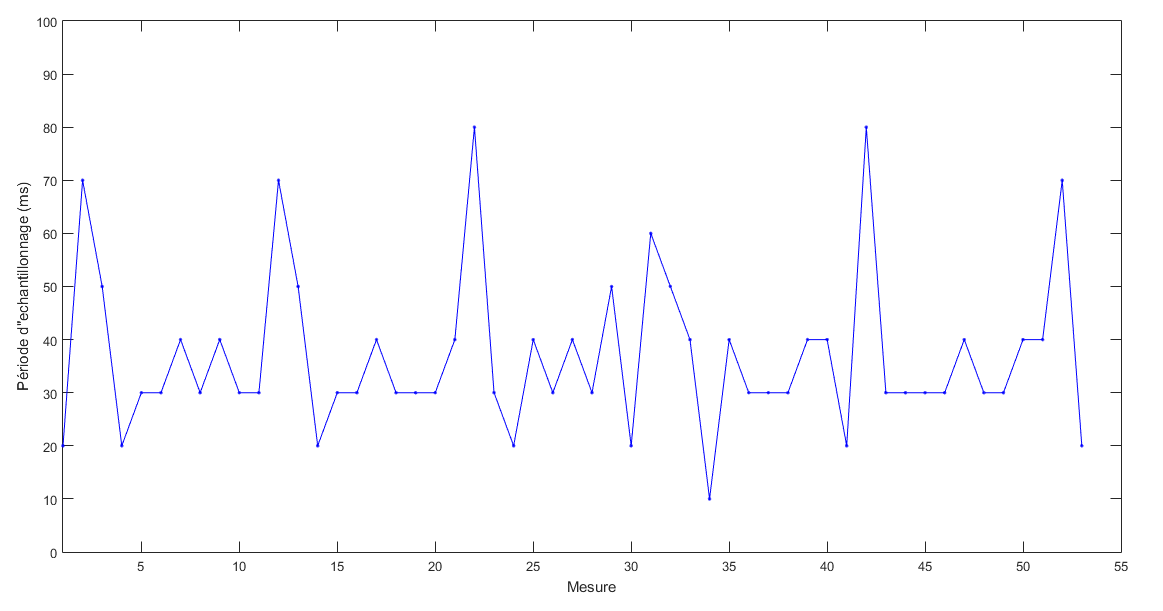
\includegraphics[scale=0.35]{kinect_periode.png}
\caption{Période d'échantillonnage de la Kinect}
\label{fig4}
\end{figure}

Le programme enregistre la position des mains de l'utilisateur dans le plan de projection 2D. Nous avons également daté chaque mesure. A la fin de la période d'enregistrement, les valeurs sont stockées dans un fichier que le programme principal pourra ensuite analyser.


\subsection{Synchronisation des mesures}

Le fait que la période d'échantillonnage du téléphone ne soit pas strictement respectée et que celle de la Kinect ne puisse pas être contrôlée nous a poussé à ne pas synchoniser les prises de mesures de manière extrêmement précise. De plus le téléphone et l'ordinateur ne dispose pas de la même horloge, ce qui aurait rendu la synchronisation très compliquée. Nous avons choisi de plutôt gérer cette synchronisation au niveau de l'analyse des mesures. La seule contrainte est que la prise de mesure commence à peu prêt au même moment sur les deux appareils. Afin d'estimer le temps mis pour démarrer un enregistrement sur le téléphone à partir du programme principal, nous avons mesuré le temps nécessaire pour l'aller-retour d'un ordre entre le PC et le téléphone. Il s'agit du temps total entre l'envoi de l'ordre et la réception de la réponse du téléphone. On peut donc considérer que le temps mis pour démarrer un enregistrement correspond à la moitié de celui-ci.

\begin{figure}[H]
\centering
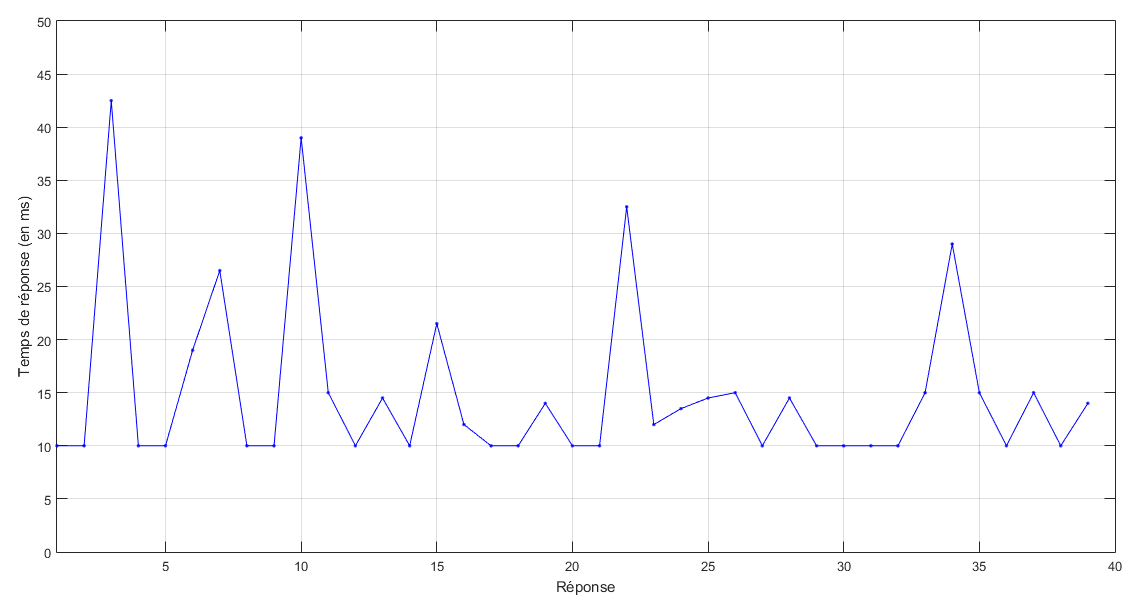
\includegraphics[scale=0.35]{temps_reponse.png}
\caption{Temps de réponse du téléphone}
\label{fig5}
\end{figure}


On voit bien que ce temps de réponse n'est pas vraiment régulier. La moyenne du temps d'envoi serait 7.5 ms.


Du côté de la Kinect, comme les deux programmes communiquent à travers une zone de même partagée, on peut considérer que l'orde de démarrage est instantané. Cependant, on a vu précédemment que la péridode d'échantillonnage de la Kinect variait entre 20 et 80 ms. Un certain délai sera donc nécessaire avant la première mesure.

Les deux appareils vont donc commencé leur prise de mesure à des instants proches mais qui peuvent différer de quelques millisecondes. Un possible décalage temporel a été pris en compte lors de l'analyse des mesures.


\subsection{Analyse des mesures}

Une fois, les enregistrements terminés, le programme principal (en Python) reçoit les différentes mesures et peut alors les traiter. Le but final étant de déterminer dans quelle main se trouvait le téléphone, nous devons comparer les accélérations du téléphone avec les positions de chaque main. Evidemment, ces deux mesures ne sont pas comparables directement et nous avons donc dû les transformer en données comparables. Pour faire cela, nous aurions pu intégrer deux fois les accélérations pour nous ramener à des positions ou même dériver deux fois les positions pour obtenir des accélérations. Cependant dériver ou intégrer des données bruitées s'avère assez problématique. Pour éviter de trop dégrader une des mesures, nous avons choisi de ramener les trois mesures à des vitesses que l'on peut, ensuite, comparer. Nous dérivons donc les positions et intégrons les accélérations.

\subsection{Mesures du smartphone}

Après une phase d'enregistrement, nous obtenons les trois valeurs d'accélération linéaire du téléphone. Ces données sont datées. Comme expliqué précédemment, la première étape a été de les projeter dans le repère "monde". Une fois dans ce repère, nous ne gardons que les axes X et Z pour obtenir les accélérations horizontales et verticales dans le plan de l'utilisateur.

\begin{figure}[H]
\centering
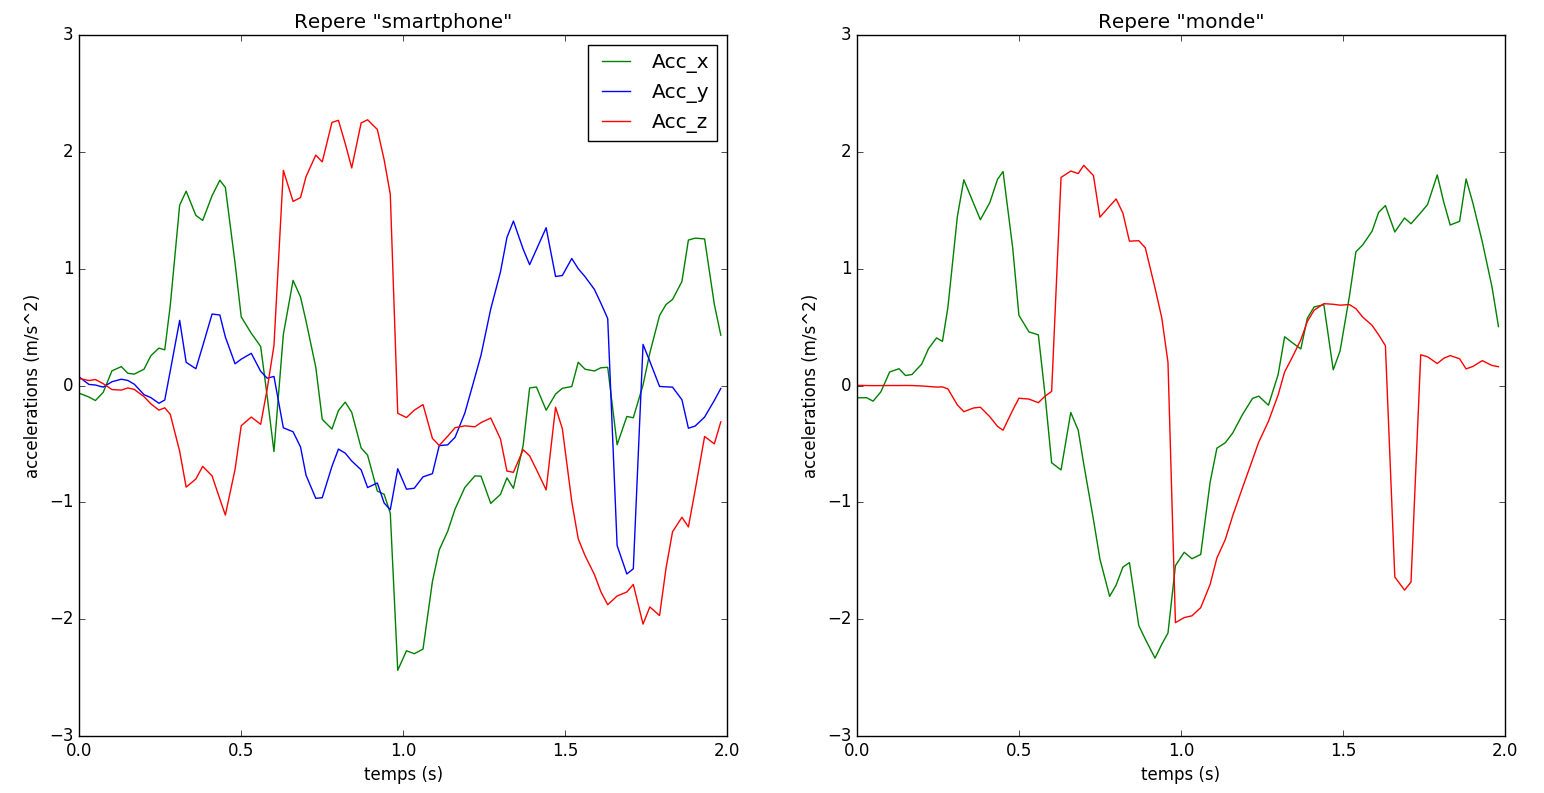
\includegraphics[scale=0.37]{repere_monde.png}
\caption{Changement de repère}
\label{fig6}
\end{figure}


Ensuite, nous avons appliqué un filtre médian qui permet de réduire le bruit des mesures.

\begin{figure}[H]
\centering
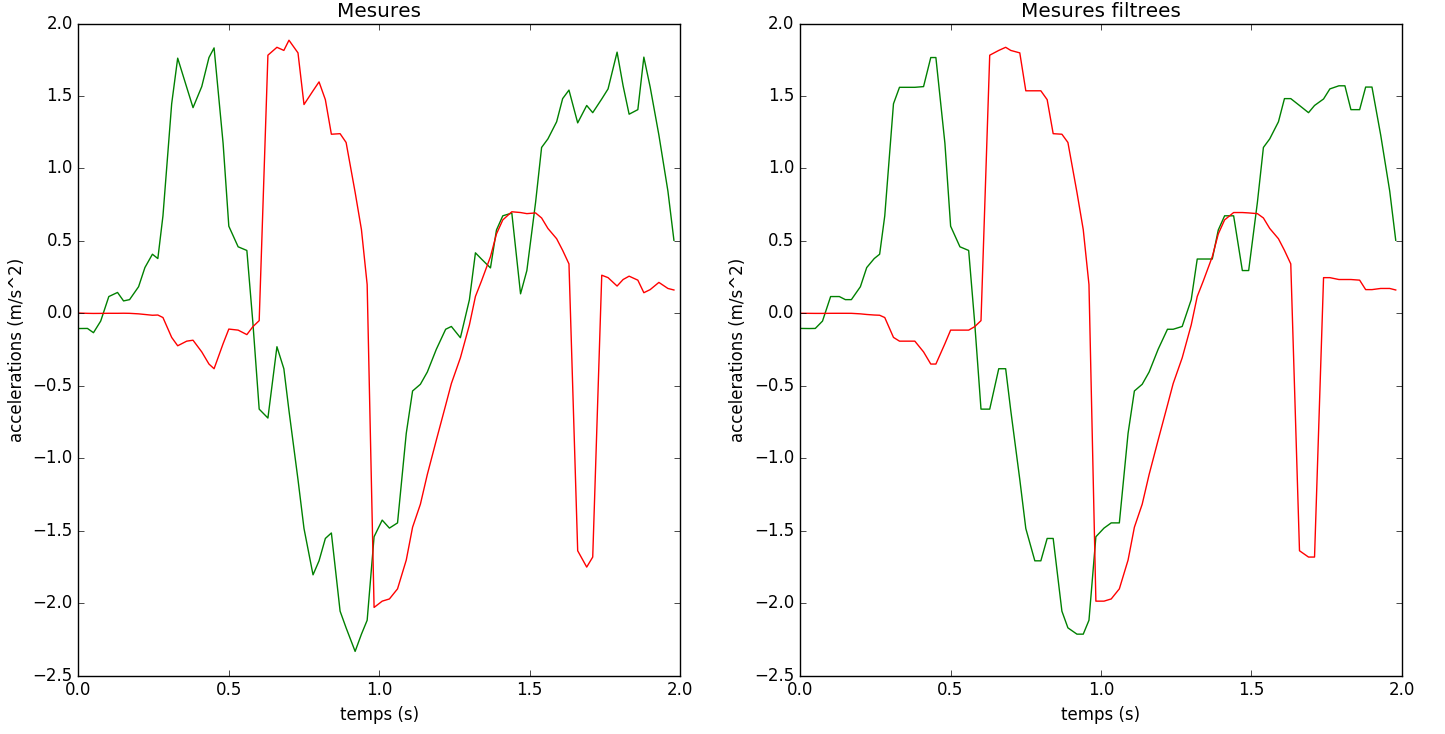
\includegraphics[scale=0.37]{mesures_filtrees.png}
\caption{Filtrage des mesures}
\label{fig7}
\end{figure}

Pour obtenir les vitesses horizontales et verticales, nous avons integré  les accélérations. Ici, les vitesses sont donc données en m/s. Cependant, le programme gérant la Kinect retourne des positions en pixels et donc les vitesses seront en pixels/s. Pour éviter des problèmes d'unités, nous avons normalisé la vitesse.


\begin{figure}[h]
\centering
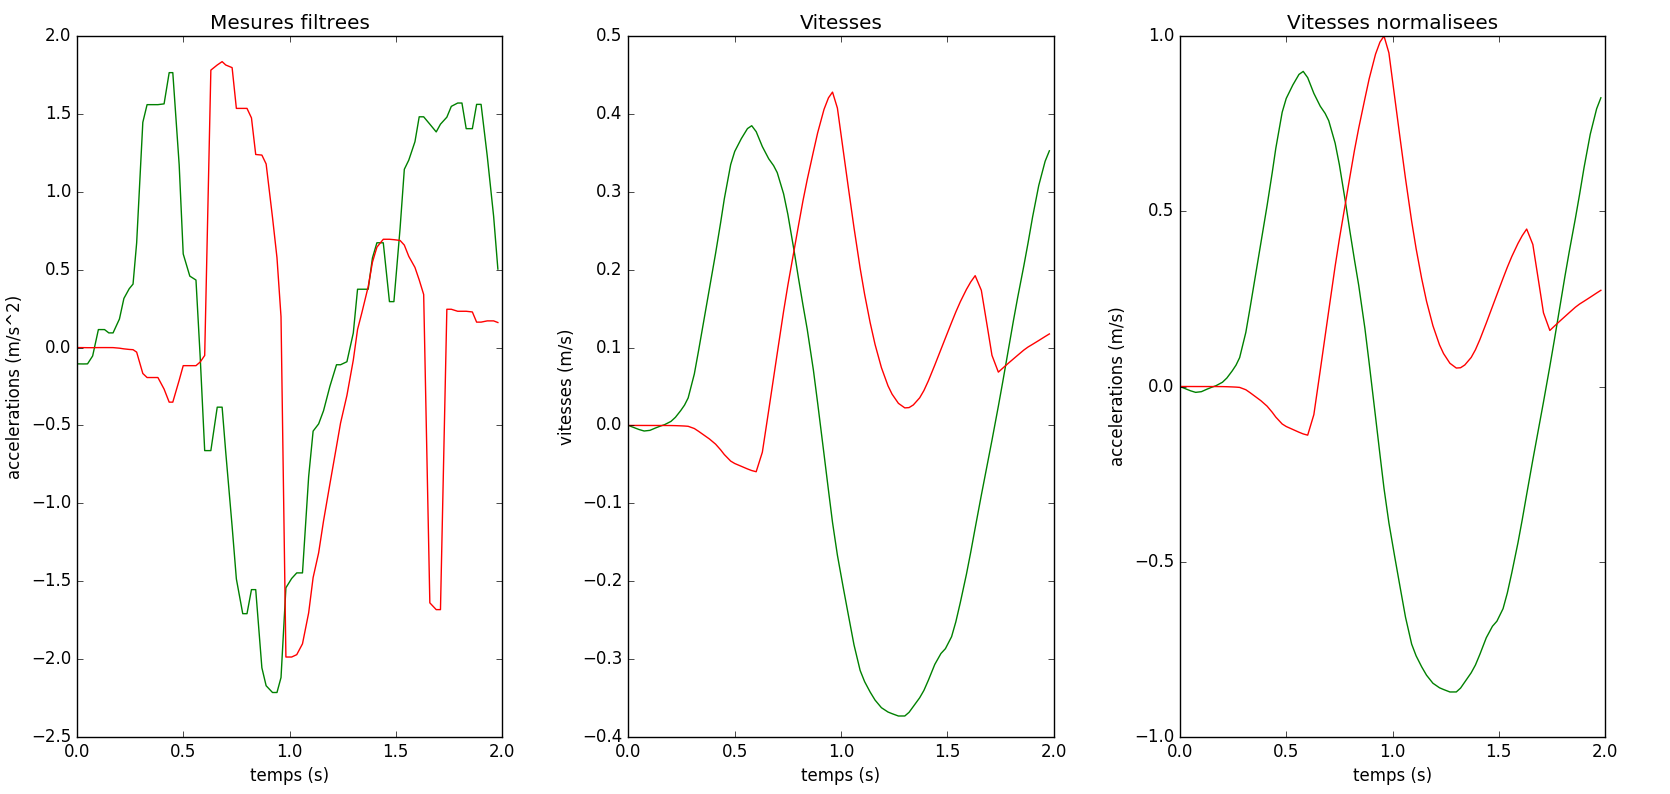
\includegraphics[scale=0.3]{vitesses_sm.png}
\caption{Intégration des accélérations pour obtenir les vitesses}
\label{fig8}
\end{figure}

\subsection{Mesures de la Kinect}

Du côté de la Kinect, nous obtenons les positions (x,y) datées de chaque main. Nous avons calculé les vitesses horizontales et verticales des mains pour chaque position en calculant :
\[V_x(t) = \frac{\Delta x}{\Delta t}=\frac{x(t)-x(t-1)}{date(t)-date(t-1)}\] 
\[V_y(t) = \frac{\Delta y}{\Delta t}=\frac{y(t)-y(t-1)}{date(t)-date(t-1)}\]

Comme pour les mesures du téléphone, nous avons utilisé un filtre médian afin de réduire le bruit et nous avons normalisé les vitesses car elles sont données en pixels/s.


\begin{figure}[H]
\centering
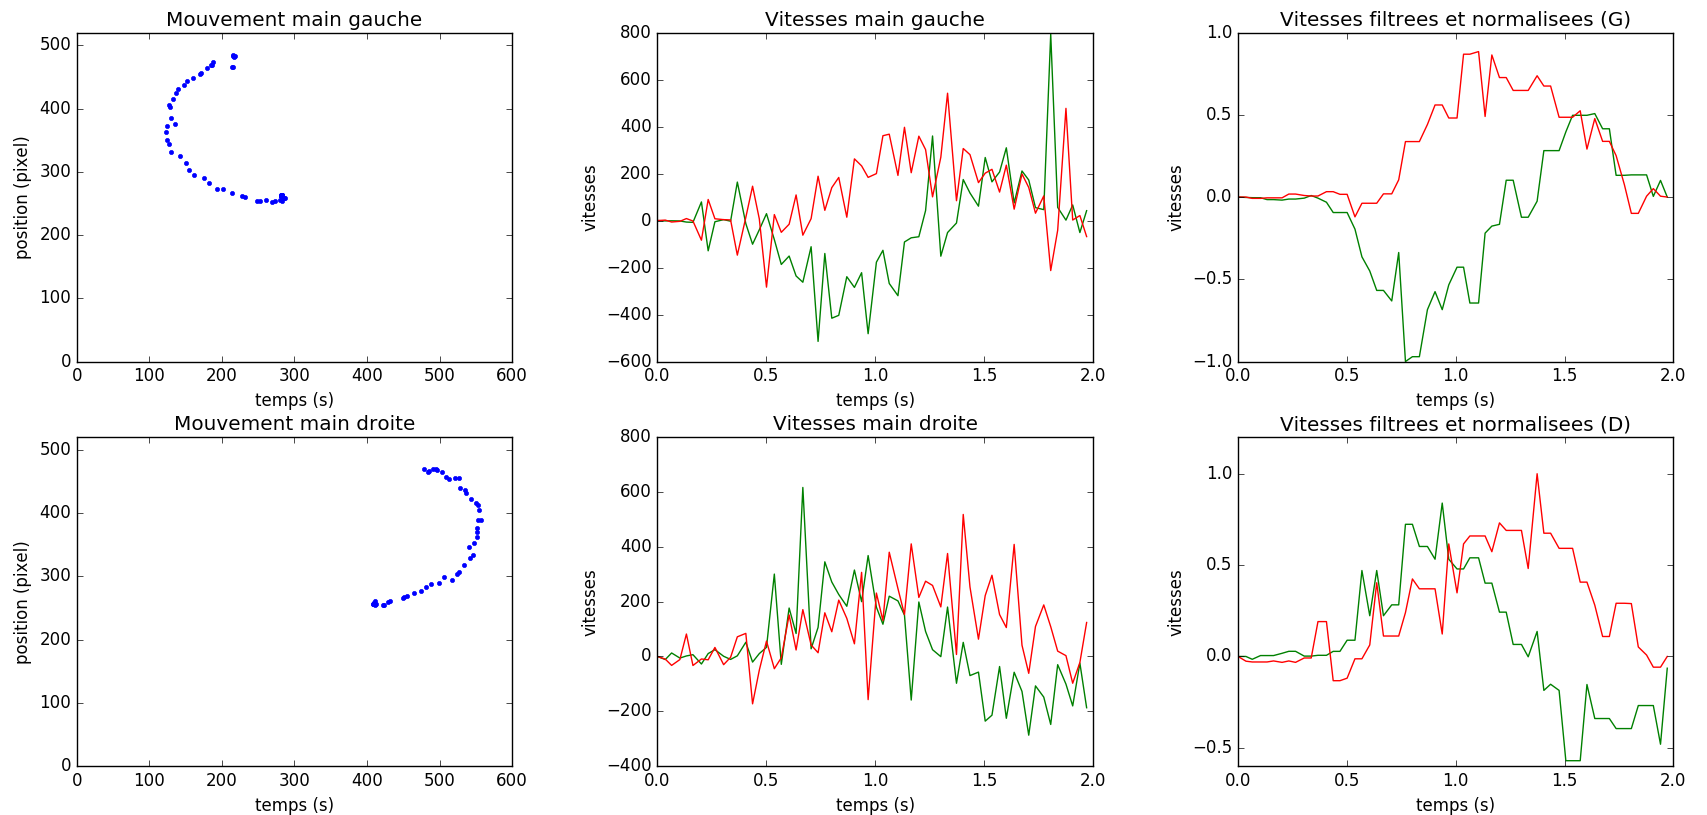
\includegraphics[scale=0.3]{kinect_pos_vit.png}
\caption{Dérivation des positions pour obtenir les vitesses des mains}
\label{fig9}
\end{figure}

\subsection{Mise en correspondance}

Une fois que l'on a obtenu les vitesses des mains ainsi que la vitesse du téléphone à différents instants, l'objectif est de les comparer pour déterminer à quelle main correspond le téléphone. Celles qui correspondent devraient être assez semblables.

Un premier problème se pose car, comme vu précédemment, les fréquences des mesures ne sont pas les mêmes entre le téléphone et la Kinect. Il est donc impossible de comparer directement les vitesses car elles ne sont prises aux mêmes instants. Pour corriger ce problème, nous avons fait une interpolation linéaire des vitesses. Comme les périodes d'échantillonnage sont assez petites (quelques millisecondes), nous considérons que la vitesse évolue de manière linéaire entre deux mesures. Avec cette interpolation, nous avons pu  ré-échantillonner les mesures à une certaine fréquence (50Hz par exemple). Cela nous permet  d'obtenir les vitesses du téléphone et des deux mains à des instants identiques.

Par exemple, voici le ré-échantillonnage de la vitesse de la main gauche. Initialement nous disposons de 60 mesures répartie de manière non régulière sur la période totale d'enregistrement. En faisant l'interpolation linéaire et en ré-échantillonnant nous obtenons 100 mesures réguilèrement réparties.

\begin{figure}[h]
\centering
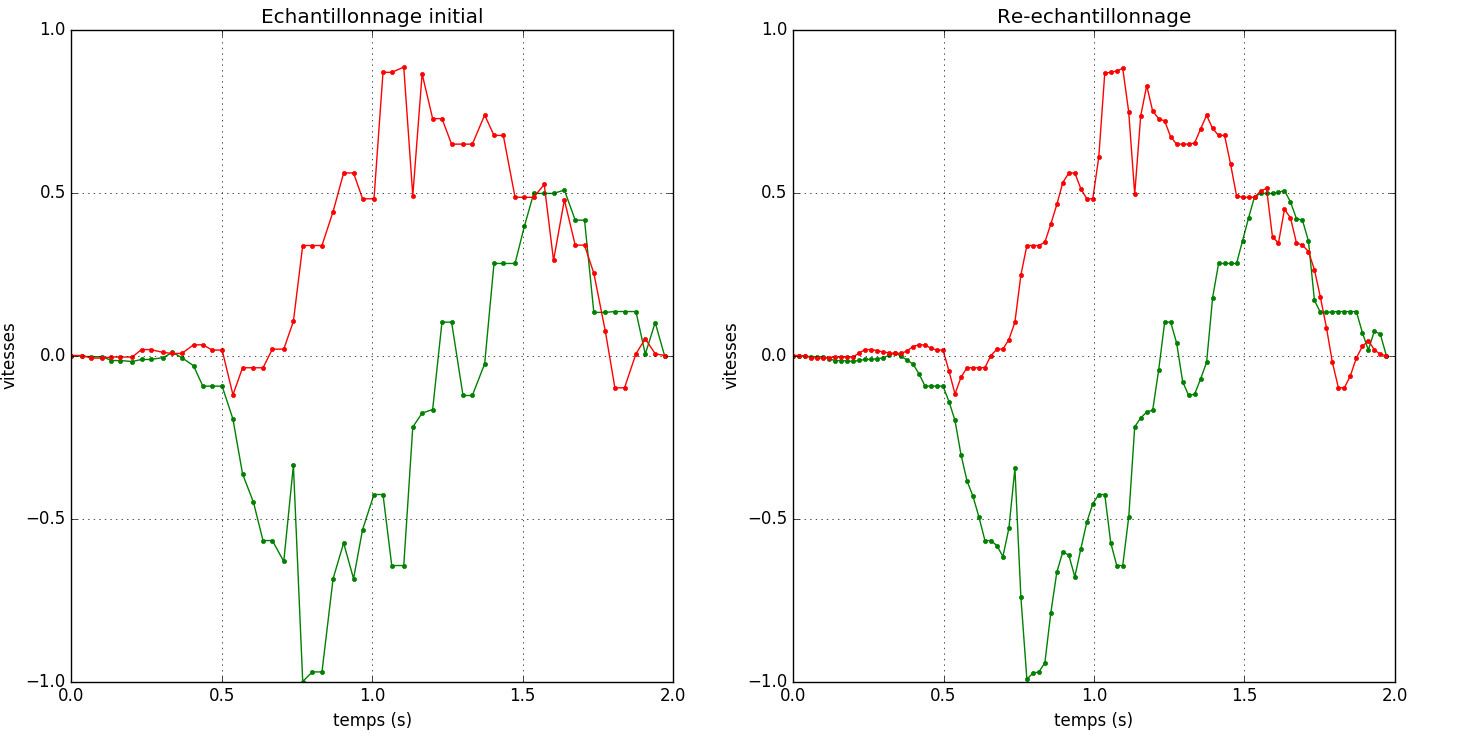
\includegraphics[scale=0.3]{reechantillonnage.png}
\caption{Ré-échatillonnage de la vitesse de la main gauche}
\label{fig10}
\end{figure}

Après cette étape, on peut donc comparer les vitesses valeur par valeur. On peut déterminer la main qui tenait le téléphone comme étant celle dont la vitesse est la plus proche de celle du téléphone en utilisant la distance Euclidienne comme critère.

En faisant, différents essais, nous avons remarqué que les mesures étaient souvent décalées de le temps. Par exemple, dans l'exemple ci-dessous, on peut voir que les courbes sont assez semblables mais qu'elles sont décalées au niveau du temps. Cela pourrait être dû au fait que nous n'avons pas pû assurer que les deux appareils commencent leur enregistrement exactement en même temps.

\begin{figure}[H]
\centering
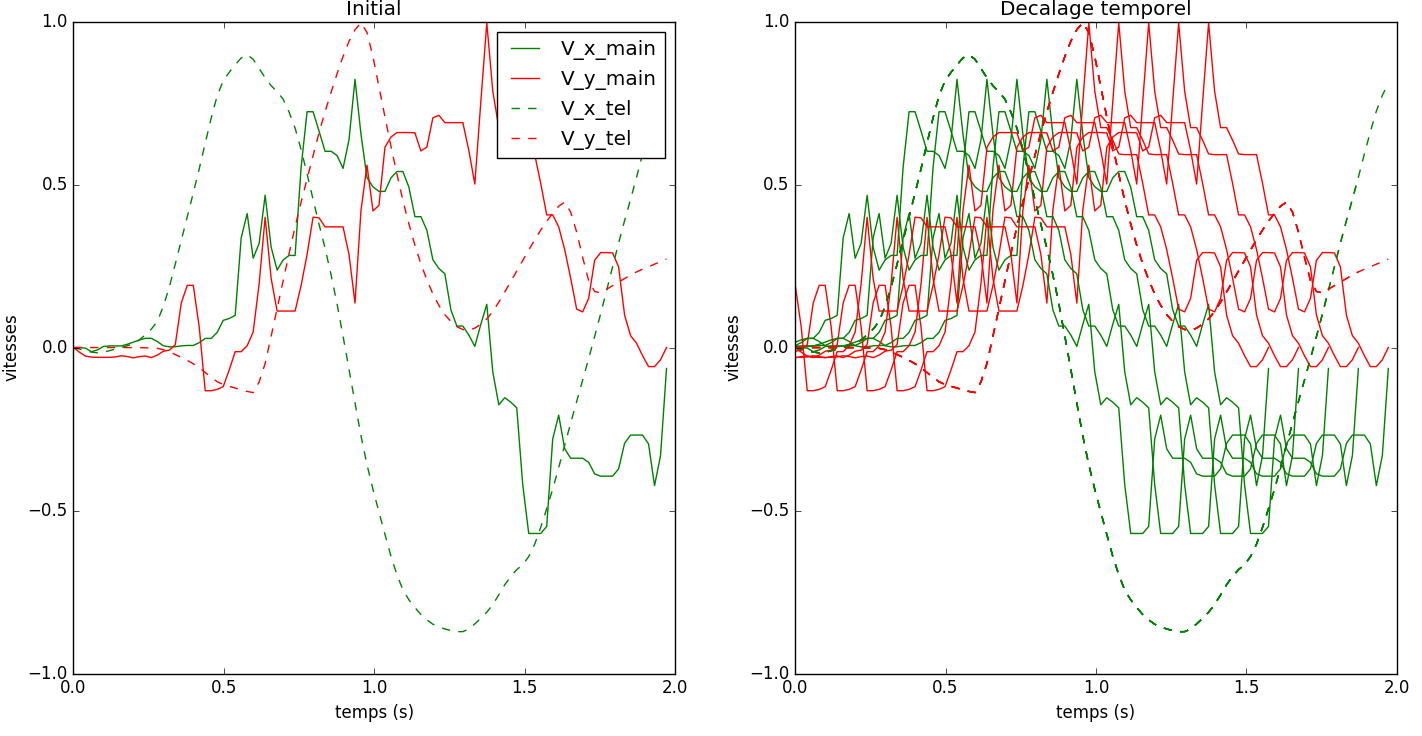
\includegraphics[scale=0.3]{decalage_tempo.png}
\caption{Recalage temporel des mesures de la Kinect}
\label{fig11}
\end{figure}


Pour résoudre ce problème, nous avons décalé les mesures de la Kinect (voir Fig\ref{fig11}) en définissant une zone de décalage maximal. Pour chaque décalage, nous calculons la distance moyenne entre les courbes et nous conservons la distance minimale. Avec ce recalage des courbes, les résultats sont bien meilleurs car la différence entre les vitesses du téléphones et celles de la bonne main est plus faible.


\section{Conclusion}
Notre programme permet donc bien de déterminer la main dans laquelle l'utilisateur tenait le téléphone. Les résultats sont assez cohérents. Nous avons débuté en spécifiant les exigences fonctionnelles et extra-fonctionnelles du produit. Puis, tout au long de la phase de développement, nous avons suivi une approche incrémentale. Par exmple, une première version utilisant la bibliothèque Qt a été développée, puis nous avons utilisé Python pour la deuxième version. Nous avons ensuite amélioré les versions au fur et à mesure, notamment en prenant en compte l'orientation du téléphone ou encore en ajoutant le recalage temporel des mesures de la Kinect lors de l'analyse.



\end{document}